\documentclass[letterpaper,10pt]{article}

\usepackage{enumitem}
\usepackage{titling}
\usepackage{listings}
\usepackage{url}
\usepackage{hyperref}
\usepackage{setspace}
\usepackage{subfig}
\usepackage{sectsty}
\usepackage{pdfpages}
\usepackage{colortbl}
\usepackage{multirow}
\usepackage{multicol}
\usepackage{relsize}
\usepackage{amsmath}
\usepackage{wasysym}
\usepackage{fancyvrb}
\usepackage[yyyymmdd]{datetime}
\usepackage{amsmath,amssymb,amsthm,graphicx,xspace}
\usepackage[titlenotnumbered,noend,noline]{algorithm2e}
\usepackage[compact]{titlesec}
\usepackage{XCharter}
\usepackage[T1]{fontenc}
\usepackage[scaled]{beramono}
\usepackage[normalem]{ulem}
\usepackage{booktabs}
\usepackage{tikz}
\usetikzlibrary{arrows,automata,shapes,trees,matrix,chains,scopes,positioning,calc}
\tikzstyle{block} = [rectangle, draw, fill=blue!20,
text width=2.5em, text centered, rounded corners, minimum height=2em]
\tikzstyle{bw} = [rectangle, draw, fill=blue!20,
text width=4em, text centered, rounded corners, minimum height=2em]

\definecolor{namerow}{cmyk}{.40,.40,.40,.40}
\definecolor{namecol}{cmyk}{.40,.40,.40,.40}
\renewcommand{\dateseparator}{-}

\let\LaTeXtitle\title
\renewcommand{\title}[1]{\LaTeXtitle{\textsf{#1}}}

\lstset{basicstyle=\footnotesize\ttfamily,breaklines=true}

\newcommand{\handout}[5]{
	\noindent
	\begin{center}
		\framebox{
			\vbox{
				\hbox to 5.78in { {\bf SE 350: Operating Systems } \hfill #2 }
				\vspace{4mm}
				\hbox to 5.78in { {\Large \hfill #4  \hfill} }
				\vspace{2mm}
				\hbox to 5.78in { {\em #3 \hfill \today} }
			}
		}
	\end{center}
	\vspace*{4mm}
}

\newcommand{\lecture}[3]{\handout{#1}{#2}{#3}{Lecture#1}}
\newcommand{\tuple}[1]{\ensuremath{\left\langle #1 \right\rangle}\xspace}

\newcommand{\Rplus}{\protect\hspace{-.1em}\protect\raisebox{.35ex}{\smaller{\smaller\textbf{+}}}}
\newcommand{\Cpp}{\mbox{C\Rplus\Rplus}\xspace}


\addtolength{\oddsidemargin}{-1.000in}
\addtolength{\evensidemargin}{-0.500in}
\addtolength{\textwidth}{2.0in}
\addtolength{\topmargin}{-1.000in}
\addtolength{\textheight}{1.75in}
\addtolength{\parskip}{\baselineskip}
\setlength{\parindent}{0in}
\renewcommand{\baselinestretch}{1.5}
\newcommand{\term}{Winter 2023}
\newcommand{\termnumeric}{1231}

\singlespace


\begin{document}

\lecture{ 29 --- Real-Time Scheduling, Windows \& UNIX }{\term}{Jeff Zarnett}

\section*{Real-Time Scheduling}
This isn't a real-time operating systems course, but I'll give you an introduction to the idea; specifically, scheduling for real-time systems. But what is a real-time system? It is one that is supposed to respond to events within a certain amount of real (wall-clock) time. There are deadlines, and there are consequences for missing deadlines. Furthermore, fast is not as important as predictable. If real time systems are of interest to you, you may wish to take some of the later embedded systems courses, or the famous CS trains course\footnote{Abandon sanity, all ye who enter here.}.

We say that a task is \textit{hard real-time} if it has a deadline that must be met to prevent an error, prevent some damage to the system, or for the answer to make sense. If a task is attempting to calculate the position of an incoming missile, a late answer is no good. A \textit{soft real-time} task has a deadline that is not, strictly speaking, mandatory; missing the deadline degrades the quality of the response, but it is not useless~\cite{osi}.

If a task is hard real-time, there are two scenarios in which it might not complete before its deadline. The first is that it is scheduled too late; like an assignment that will take two hours to complete being started one hour before the deadline. If that is the case, the system will likely reject the request to start the task, or perhaps never schedule the task to run at all. Why waste computation time on a task that will not finish in time? The second scenario is that at the time of starting, completion was possible, but for whatever reason (e.g., other tasks with higher priority have occurred) it is no longer possible to meet the deadline. In that case, execution of the task may be terminated partway through so that no additional effort is wasted on a task that cannot be completed.

As a general note, most of the operating systems you are familiar with (standard Desktop/Server Linux, Mac OS, Windows) are not very suitable to real time systems. They make few guarantees, if any, about service. When there are consequences for missing deadlines, this kind of thing matters. This was, as we already discussed, a reason why Java is not a very good choice for a real-time system: the garbage collector runs whenever it pleases and can ``stop the world'' (halt all execution) until that is finished. And how long is that going to take? Nobody knows.

In Windows you can set a high priority (e.g. level 31) to a process and it calls the priority ``Realtime'', but please don't be fooled: this does not mean it guarantees it will make a particular deadline.

\subsection*{Timeline Scheduling}
If a process or task recurs at regular intervals, it is \textit{periodic} -- repeats at a fixed period. Periodic tasks are very common: check a sensor, decode and display a frame of video to a screen, keep the wifi connection alive, etc.

Consider a periodic task to have two attributes: $\tau_{k}$, the period (how often the task occurs) and $c_{k}$, the computation time (how long, in the worst case, the task might execute). In real-time systems we are usually pessimists and care almost exclusively about the worst case scenario. We can calculate the processor utilization of periodic tasks according to the following formula, to get the long-term average of processor utilization $U$~\cite{mte241}:

\begin{center}
$U = \sum\limits_{k=1}^n\dfrac{c_{k}}{\tau_{k}}$
\end{center}

If $U > 1$, it means the system is overloaded: there are too many periodic tasks and we cannot guarantee that the system can execute all tasks and meet the deadlines. Otherwise, we will be able to devise a schedule of some sort that makes it all work.

If the only tasks in the system are periodic ones, then we can create a fixed schedule for them. This is what the university administrators do when they create the schedule of classes for a given term. Every Monday, for example, from 13:30-14:50, course SE~350 (a ``process'', if you will) takes place in classroom STC~0050 (a resource). There is no way to have two classes in the same lecture hall at the same time, so if there are more requests for room reservations than rooms and time slots available, it means some requests cannot be accommodated.

A world in which all the tasks are periodic and behave nicely is, well, a very orderly world (and that has its appeal). Unfortunately, the real world is not so accommodating most of the time. So we will need to deal with tasks that are not periodic, which we can categorize as \textit{aperiodic} or \textit{sporadic}.

Aperiodic tasks are ones that respond to events that occur irregularly. There is no minimum time interval between two events; therefore it would be very difficult to make a guarantee that we will finish them before the next one occurs, so they are rarely hard real-time (hard deadlines). Tasks like this should be scheduled in such a way that that they do not prevent another task with a hard deadline from missing its deadline. As an example, if we expect an average arrival rate of 3 requests per second, there is still a 1.2\% chance that eight or more requests appear within 1~second. If so, there is not much we can do to accommodate them all (most likely)~\cite{mte241}.

Sporadic tasks are aperiodic, but they require meeting deadlines. To make such a promise we need a guarantee that there is a minimum time $\tau_{k}$ between occurrences of the event. Sporadic tasks can overload the system if there are too many of them, and if that is the case, we must make decisions about what tasks to schedule and which ones will miss their deadlines. If we know a task will not make its deadline, we will likely not even bother to schedule it (why waste the time on a task where the answer will be irrelevant?)~\cite{mte241}.

So, these aperiodic and sporadic tasks really mess with timeline scheduling. This unpredictability makes it hard to create a simple timetable and follow it, just as we would expect when it comes to assigning classes and rooms. 

If we have pre-emptive scheduling, then we can examine two optimal alternatives. They are called optimal because they will ensure a schedule where all tasks meet their deadlines, not because they are the ideal algorithms.

\subsection*{Earliest Deadline First}

The earliest deadline first algorithm is, presumably, very familiar to students. If there is an assignment due today, an assignment due next Tuesday, and an exam next month, then you may choose to schedule these things by their deadlines: do the assignment due today first. After completing an assignment, decide what to do next (probably the new assignment, but perhaps a new task has arrived in the meantime?) and get on with that.

The principle is the same for the computer. Choose the task with the soonest deadline; if there is a tie, then random selection between the two will be sufficient (or other criteria may be used, if desired). If there exists some way to schedule all the tasks such that all deadlines are met, this algorithm will find it. If a task is executing because its deadline is the earliest and another task arrives with a sooner deadline, then preemption means the currently executing task should be suspended and the new task scheduled. This might mean a periodic task being preempted by an aperiodic or sporadic task~\cite{mte241}.

\subsection*{Least Slack First}
A similar algorithm to earliest deadline first, is least slack first. The definition of \textit{slack} is how long a task can wait before it must be scheduled to meet its deadline. If a task will take 10~ms to execute and its deadline is 50~ms away, then there are (50 - 10) = 40~ms of slack time remaining. We have to start the task before 40~ms are expired if we want to be sure that it will finish. This does not mean, however, that we necessarily want to wait 40~ms before starting the task (even though many students tend to operate on this basis). All things being equal, we prefer tasks to start and finish as soon as possible. It does, however, give us an indication of what tasks are in most danger of missing their deadlines and should therefore have priority.


\section*{Commercial OS Scheduling Algorithms}

In this section we will examine how real commercial operating systems schedule their processes and threads. We will examine UNIX, Windows, and finally, Linux scheduling. We will see what approaches are used and what is interesting or novel about them.

\subsection*{Traditional UNIX}

The traditional UNIX scheduling is really ancient; as in System V R3 and BSD 4.3. It was replaced in SVR4 (which had some real-time support). The information about the traditional UNIX scheduler comes primarily from~\cite{osi}.

The routine is a multilevel feedback system using Round Robin within each of the priority queues. Time slicing is implemented and the default time slice is a (very long) 1 second. So if a process does not block or complete within 1~s, then it will be preempted. Priority is based on the process type as well as the execution history.

Processor utilization for a process $j$ is calculated for an interval $i$ by the following formula:

\begin{center}
$CPU_{j}(i) = \dfrac{CPU_{j}(i - 1)}{2}$
\end{center}

And the priority is for process $j$ at interval $i$ is calculated by the formula:

\begin{center}
$P_{j}(i) = B_{j} + \dfrac{CPU_{j}}{2} + N_{j}$
\end{center}

where $B_{j}$ is the base priority of process $j$ and $N_{j}$ is the ``nice'' value of process $j$. The ``nice'' value is a UNIX way to allow a user to voluntarily reduce the priority of a process to be ``nice'' to other users (but honestly, who uses this?)~\cite{mos}. Actually, the answer to that question is: system administrators. An admin can ``re-nice'' a process and make it somewhat nicer than it would otherwise be.

The $CPU$ and $N$ components of the equation are restricted to prevent a process from migrating outside of its assigned category. A process is assigned to a given category based on what kind of process it is. To put it in simple terms, the OS puts its own needs first and tries to make the best use of resources it can. From highest to lowest priority, the categories are:

\begin{enumerate}
	\item Swapper (move processes to and from disk)
	\item Block I/O device control (e.g., disk)
	\item File manipulation
	\item Character I/O device control (e.g., keyboard)
	\item User processes
\end{enumerate}

Yes, unfortunately, user processes get piled at the bottom of the list. The use of the hierarchy should provide for efficient use of I/O devices and tends to penalize processor-bound processes at the expense of I/O bound processes. This is beneficial, because CPU-bound processes should be able to carry on executing when an I/O-bound process waits for the I/O operation to complete, but when an I/O operation is finished, we would like to start the next I/O operation so the I/O device is not waiting. This strategy is reasonably effective for a general-purpose, time-sharing operating system.

\subsection*{Windows}

Windows schedules threads using a priority-based, preemptive scheduling algorithm, ensuring that the highest priority thread runs. The official name for the selection routine is the \textit{dispatcher}. A thread will run until it is preempted, blocks, terminates, or until its time slice expires. If a higher priority thread is unblocked, it will preempt a lower priority thread. Windows has 32 different priority levels, the regular (priority 1 to 15) and real-time classes (16 to 31). A memory management task runs at priority 0. The dispatcher maintains a queue for each of the scheduling priorities and goes through them from highest to lowest (yes, in Windows, higher numbers are higher priorities) until it finds something to do (and if there is nothing else currently ready, the System Idle Process will ``run'')~\cite{osc}.

There are six priority classes you can set a process to via Task Manager, from highest to lowest:
\begin{enumerate}
	\item Realtime
	\item High
	\item Above Normal
	\item Normal
	\item Below Normal
	\item Low
\end{enumerate}

A process is usually in the Normal class. Within that class there are some more relative priorities. Unless it is in the real-time category, the relative priority can change. The details are summarized in the table below:

\begin{center}
	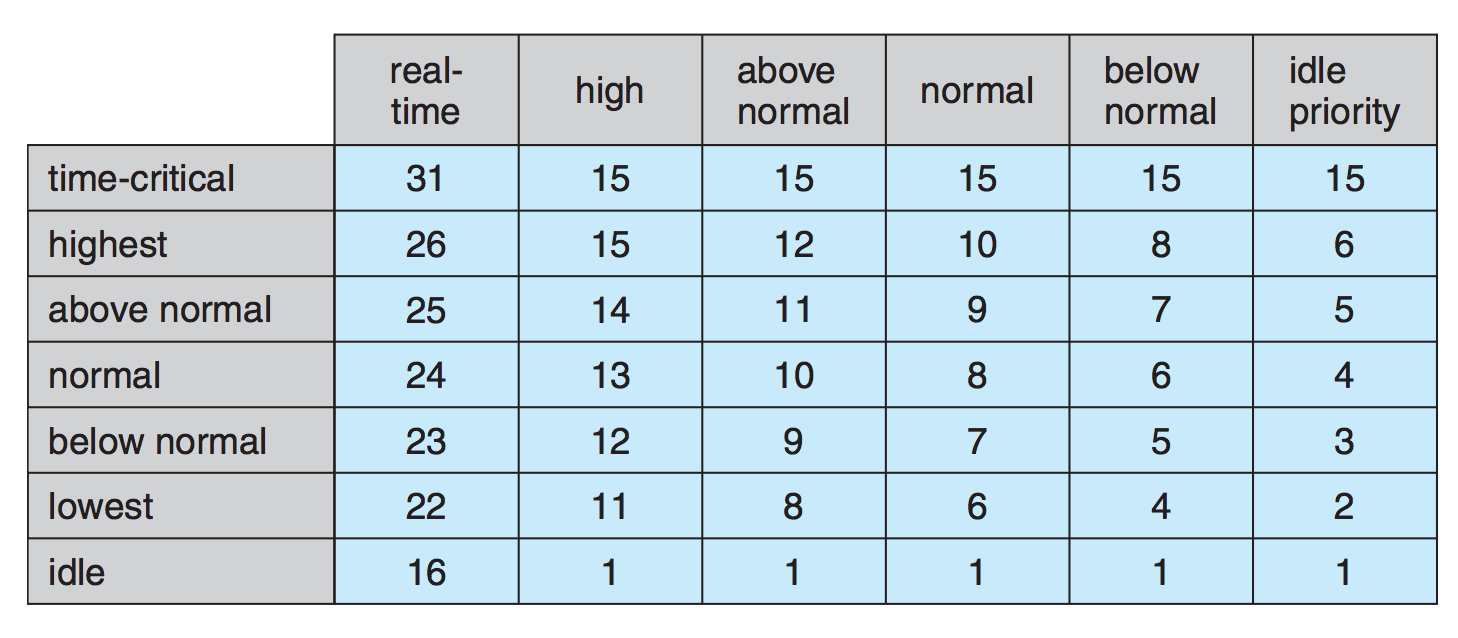
\includegraphics[width=0.7\textwidth]{images/windows-thread-priorities.png}\\
	Windows thread priorities~\cite{osc}.
\end{center}

If a process reaches the end of a time slice, the thread is interrupted, and unless it is in the real-time category, its priority will be lowered, to a minimum of a of the base priority of each class. When a process that was blocked on something (e.g., a wait or I/O), its priority is temporarily boosted (unless it is real-time, in which case it cannot be boosted). The amount of the boost depends on what the event was: a process that was waiting for keyboard input gets a bigger boost than one that was waiting for a disk operation, for example~\cite{osc}. 

The operating system also gives a priority to whatever process is running in the selected foreground window. This is different from foreground vs. background processes as discussed earlier, because the definition of a foreground process was one that was user-interactive. Here, the distinction is which of the user-interactive processes is currently ``on top'' in the UI. Not only does this process get a priority boost, but it also gets longer time slices. This can be disabled, if so desired, but it really highlights the different heritages of Windows and UNIX. UNIX was originally a time-sharing system with multiple users and lots of processes; Windows was originally a single-user desktop operating system doing one or maybe a few things at a time.


\bibliographystyle{alphaurl}
\bibliography{350}


\end{document}